\section[Git]{Git}
\begin{frame}
	\frametitle{About git}
	\begin{columns}
		\begin{column}{0.7\textwidth}
			\begin{itemize}[<+->]
				\item Developed by the team behind Linux
				\item used by companies such as:
				\begin{itemize}[<+->]
					\item Linux
					\item Microsoft
					\item Google
					\item Android
					\item Facebook
					\item Twitter
					\item Linkedin
				\end{itemize}
			\end{itemize}
		\end{column}
		\begin{column}{0.3\textwidth}
			
\includegraphics{./pictures/Git-Icon.eps}
		\end{column}
	\end{columns}
\end{frame}
\begin{frame}
	\frametitle{Getting started with git}
	\begin{columns}
		\begin{column}{0.5\textwidth}
			\begin{itemize}[<+->]
				\item Download git
					\begin{itemize}[<+->]
							\item \url{www.git-scm.com}
							\item Your favourite package manager
					\end{itemize}
				\item Get a server:
					\begin{itemize}[<+->]
						\item Set up yourself
						\item GitHub
						\item BitBucket
				\end{itemize}
				\item Get a client:
					\begin{itemize}[<+->]
						\item Command line is already included
						\item GitKraken
						\item Check out list at \url{www.git-scm.com/downloads/guis}
					\end{itemize}
				\end{itemize}
			\end{column}
			\begin{column}{0.5\textwidth}
					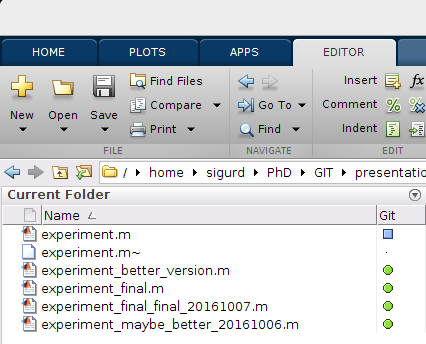
\includegraphics[width=\textwidth]{./pictures/matlab.png}
			\end{column}
	\end{columns}
\end{frame}
\begin{frame}
	\frametitle{GitHub}
	\begin{columns}
		\begin{column}{0.7\textwidth}
			\begin{itemize}[<+->]
				\item Largest host for git repositories
				\item For developers a git page is sometimes as important as a CV
				\item You can have as many open repositories you want free.
				\item Closed source projects cost money
				\item You can request an academic account at \url{https://education.github.com/}
					\begin{itemize}[<+->]
						\item You get five closed source projects for free
						\item Maybe other stuff too
					\end{itemize}
				\item Wiki for your project
				\item Place to discuss your project and fill bug reports
				\item Integrates with many cool services
			\end{itemize}
		\end{column}
		\begin{column}{0.3\textwidth}
			
\includegraphics[width=\textwidth]{./pictures/GitHub.png}
		\end{column}
\end{columns}
\end{frame}
\begin{frame}
	\frametitle{BitBucket}
		\begin{itemize}[<+->]
			\item More or less same features as GitHub
			\item Wiki, bug reporting etc. different integrated services
			\item Free closed source repositories
			\item With git it is easy to change the remote, try both GitHub and BitBucket
		\end{itemize}
\end{frame}
